\documentclass[12pt]{article}

\usepackage[margin=1in]{geometry}

\usepackage{setspace}
\singlespacing

\usepackage{mathtools}

\usepackage{enumerate}

\usepackage{graphicx}

\usepackage{verbatim}
\usepackage{empheq} %para colocar \boxed em \begin{align}

\usepackage[utf8]{inputenc}    %esses tres sao
\usepackage[T1]{fontenc}       %necessarios
\usepackage[portuguese]{babel} %para usar palavras com acento

\usepackage{indentfirst}

\usepackage{float}

\title{Minicurso de \LaTeX \\
Exemplos}
\author{Os Três Patetas}
\date{\today}

\begin{document}
\maketitle

\section{MODULO II - Elementos do Texto}

\subsection{Criando Títulos e Subtítulos}

\begin{figure}[H]
\centering
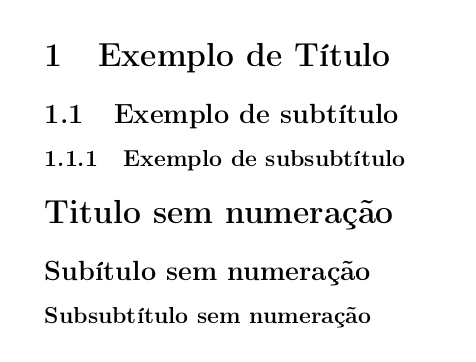
\includegraphics[scale=0.8]{exemplo_titulos.png}
\caption{Exemplo de títulos}
\end{figure}

O código para o exemplo anterior:
\begin{verbatim}
\begin{document}

\section{Exemplo de Título}

\subsection{Exemplo de subtítulo}

\subsubsection{Exemplo de subsubtítulo}

\section*{Titulo sem numeração}

\subsection*{Subítulo sem numeração}

\subsubsection*{Subsubtítulo sem numeração}

\end{document}
\end{verbatim}


\subsection{Modificadores de Texto}

Este é um exemplo de texto em \textbf{Negrito} e este é um exemplo de texto em \textit{Itálico}.

Código para o exemplo:
\begin{verbatim}
Este é um exemplo de texto em \textbf{Negrito} 

e este é um exemplo de texto em \textit{Itálico}.
\end{verbatim}

\subsection{Espaçamento}

\subsection{Inserindo Tabelas}

\begin{verbatim}
\begin{table}[h]
\begin{tabular}{c|c} 
   \toprule
    \textbf{RS}             &\textbf{Temperatura Máxima} ($^{\circ}C)$\\
   \midrule
   Porto Alegre             &39\\ \hline
   Santa Maria              &40\\ \hline
   Rio Grande               &40\\ \hline
   Pelotas                  &40\\ \hline
   Caxias do Sul            &38\\ \hline 
   \bottomrule
\end{tabular}
\end{table}
\end{verbatim}

\subsection{Ambientes}




\end{document}